\documentclass[11pt,a4paper]{article}
\usepackage{fontspec}
\setmainfont{TeX Gyre Pagella}
\newfontfamily\headfont{Inter}[UprightFont=*-ExtraBold,BoldFont=*-ExtraBold,Extension=.otf,Path=/usr/share/fonts/opentype/inter/]
\usepackage[a4paper,margin=2.3cm]{geometry}
\usepackage{graphicx,booktabs,float,caption,array,xcolor,longtable}
\usepackage{xurl}
\usepackage[hidelinks]{hyperref}
\usepackage{titlesec}
\usepackage[round]{natbib}
\usepackage{setspace}
\setstretch{1.05}
\renewcommand{\topfraction}{0.9}
\renewcommand{\bottomfraction}{0.8}
\renewcommand{\textfraction}{0.1}
\renewcommand{\floatpagefraction}{0.75}
\setlength{\parindent}{0pt}
\setlength{\parskip}{0.55em}
\titleformat{\section}{\headfont\Large}{\thesection}{0.8em}{}
\titleformat{\subsection}{\headfont\large}{\thesubsection}{0.8em}{}
\captionsetup{font=small,labelfont=bf}
\urlstyle{same}
\hypersetup{pdftitle={Islands on Land},pdfauthor={Tristan Hotham}}

\begin{document}
\begin{center}
{\Large\bfseries Islands on Land\par}
\vspace{0.4em}
{\large Enclaves, Exclaves, Tripoints and Other Oddities of the World's Borders:\\a Catalogue from Wikipedia Measured Against Natural Earth\par}
\vspace{1.2em}
{\large Tristan Hotham\par}
\vspace{0.3em}
{\small Independent researcher\\
ORCID: 0000-0003-4931-9349\\
DOI: https://doi.org/10.5281/zenodo.23873011\par}
\vspace{0.8em}
2026
\end{center}

\begin{quote}
\small
\begin{center}\textbf{Abstract}\end{center}
I compile the national-level border oddities listed in English Wikipedia (true enclaves, enclaved countries, exclaves, semi-enclaves and semi-exclaves, pene-exclaves, divided islands, former enclaves, condominiums and unclaimed land) and compare them with what can be computed from Natural Earth's 1:10m map of the world's countries. Wikipedia lists 42 true international enclaves, pieces of one country entirely surrounded by one other, in 85 separate pieces, owned by 24 countries; Germany owns the most entries (6) and Belgium the most pieces (22, all at Baarle). Their areas run from 16,000 square metres (Rückschlag) to 234 km² (Sokh) on land, and the enclaved countries reach 30,355 km² (Lesotho). Only 17 of the 42 appear as separate pieces in Natural Earth. From Natural Earth's shared boundary vertices I find 167 international tripoints and one quadripoint, at Kazungula, where Wikipedia's sources describe two tripoints about 100 to 150 m apart. China has the most tripoints (15); China and Russia have the most neighbours (14 each). Natural Earth and Wikipedia agree on the number of neighbours for 150 of 160 countries, and most disagreements are themselves oddities. Treating the Caspian as a lake, 45 countries are landlocked and two, Liechtenstein and Uzbekistan, are doubly landlocked. Natural Earth contains 50 detached pieces of countries that touch another country, 13 of them enclaves. All borders are Natural Earth's de facto lines and Wikipedia's descriptions; neither is an endorsement of any territorial claim.

\textbf{Keywords:} political geography; enclaves; exclaves; tripoints; land borders; landlocked countries; Natural Earth; Wikipedia; open data; mapping
\end{quote}

\section{Introduction}
Most of the world's land is divided into countries whose territory is a single connected piece, or a mainland with islands. The exceptions are few but persistent, and they attract attention out of proportion to their size: a Belgian house number on one half of a front door in a Dutch town, a field in Bengal that belonged to India while surrounded by Bangladesh, surrounded by India, surrounded by Bangladesh, or an island in the Bidasoa that France and Spain govern in turn. They are the residue of medieval land deals, colonial treaties written from poor maps, railway lines, and choices made by villagers about which ruler to follow \citep{wlist,wenclave}.

There is no official register of such places. The most complete public catalogue is English Wikipedia's List of enclaves and exclaves \citep{wlist}, together with articles on individual cases. Separately, Natural Earth's 1:10m countries \citep{naturalearth} are the standard free outlines used in countless maps. This paper does three things. It turns Wikipedia's national-level lists into a structured, located catalogue. It computes from Natural Earth what can be computed by machine: neighbours, border lengths, tripoints, detached pieces of countries and landlocked status. And it compares the two, which shows both how much of the world's border geography a generalised map leaves out and where the map adds oddities of its own. The paper accompanies an interactive map with a tour of 15 cases (\url{https://maps.tristanhotham.com/border-oddities/}).

\section{Data}
\textbf{Wikipedia.} I use 35 English Wikipedia articles saved as parsed HTML with their revision ids (listed in the references): the List of enclaves and exclaves; the articles on enclaves and exclaves, Baarle-Hertog and Baarle-Nassau, the India and Bangladesh enclaves and Dahagram-Angarpota, tripoints, the list of tripoints and quadripoints, condominiums, terra nullius, landlocked countries, the list of countries by land borders and the list of countries with one neighbour; and the articles on each place visited by the tour. The list article has tables for national and sub-national enclaves and exclaves (with area, owner, surrounding country and coordinates as a geo microformat) and bulleted lists for semi-enclaves, pene-exclaves and divided islands.

\textbf{Wikidata.} A Wikidata query of items that are instances of enclave and related types returned 2,739 rows for 32 item types, most of them ghettos, ethnic quarters and townships. 178 items are typed as enclaves; 29 match an entry in Wikipedia's national-level list, and 127 sub-national enclaves with coordinates are kept as a separate map layer.

\textbf{Natural Earth.} Natural Earth 1:10m admin-0 countries (258 features, 4,274 polygons) supply the geometry, and its 1:10m populated places the capitals used to choose each country's main part. Natural Earth draws de facto lines and marks some areas, including Bir Tawil and the Siachen Glacier, as indeterminate zones.

\section{Methods}
\subsection{The catalogue}
From Wikipedia's list I take the national-level sections only. Each table row becomes one entry: true enclaves (enclaves that are also exclaves), enclaved countries, exclaves that are not enclaves, and historic enclaves. 16 rows describing pockets of high seas surrounded by exclusive economic zones are set aside. Each bulleted item in the national-level lists of semi-enclaves and semi-exclaves, pene-exclaves and divided islands becomes one entry. The number of separate pieces in a table entry is read from the entry (for example, Baarle-Hertog's 22 parcels). Entries are placed by the table's coordinates; list items by coordinates written in the item, by the infobox of the article about the place, or by the representative point of the Natural Earth piece that is the place; otherwise they are kept but not mapped. Condominiums come from Wikipedia's table of current condominiums and are mapped where a source gives a position. The parcel tables for Baarle and the tables of former India and Bangladesh enclaves supply areas for the size comparison. 98 sentences quoted in the text are checked word for word against the saved articles by the code.

\subsection{Natural Earth topology}
Each Natural Earth feature is assigned to a country: its sovereignty group, so that Hong Kong and Macao count with China, Gibraltar and the Cyprus base areas with the United Kingdom, and Saint-Martin with France. Natural Earth's de facto units (Kosovo, Northern Cyprus, Somaliland, Taiwan and Western Sahara) are kept as they are, and Palestine, which Natural Earth groups with Israel, is kept separate. Indeterminate zones are not countries. Neighbouring polygons share their vertices exactly, so each polygon edge (consecutive vertices rounded to $10^{-7}$ degrees) records the countries on its two sides: no edge is shared by more than two polygons. An edge between two countries is land border, measured on the WGS84 ellipsoid; an edge with one country is coast, unless it faces water enclosed by land (a hole in the union of all land, of which the largest is the Caspian Sea, 397,054 km²), in which case it is lake shore. A tripoint is a vertex on the boundary of three countries.

\subsection{Detached pieces and landlocked countries}
A country's polygons are joined into pieces wherever they share an edge; touching at a single point does not join them. The main piece is the largest piece containing the country's principal feature, unless the piece containing the capital is at least half its size (so Peninsular Malaysia rather than Malaysian Borneo, and Jutland rather than Zealand). Every other piece that shares land border with another country is classified: an enclave if it has no sea coast and one neighbour; a landlocked exclave if it has no sea coast and several; a coastal exclave if it has a sea coast and lies on a landmass of more than two million km²; and otherwise part of a shared island. A country is landlocked if it has no sea coast, and doubly landlocked if all its neighbours are landlocked as well.

\section{Results}
\subsection{The catalogue}
The catalogue has 188 entries, 107 of them mapped (Figure~\ref{fig:map}). Wikipedia lists 42 true enclaves at national level, 32 on land and 10 islands or water areas, in 85 pieces, owned by 24 countries and surrounded by 24 (Table~\ref{tab:enclaves}, Figure~\ref{fig:owners}). It also lists 3 enclaved countries, 4 exclaves that are not enclaves, 17 semi-enclaves and semi-exclaves, 62 pene-exclaves and 36 divided islands, as well as 214 sub-national table rows, which are counted but not mapped. 51 pene-exclaves, 17 divided islands and 1 semi-exclave could not be placed from the sources.

\begin{figure}[tbp]\centering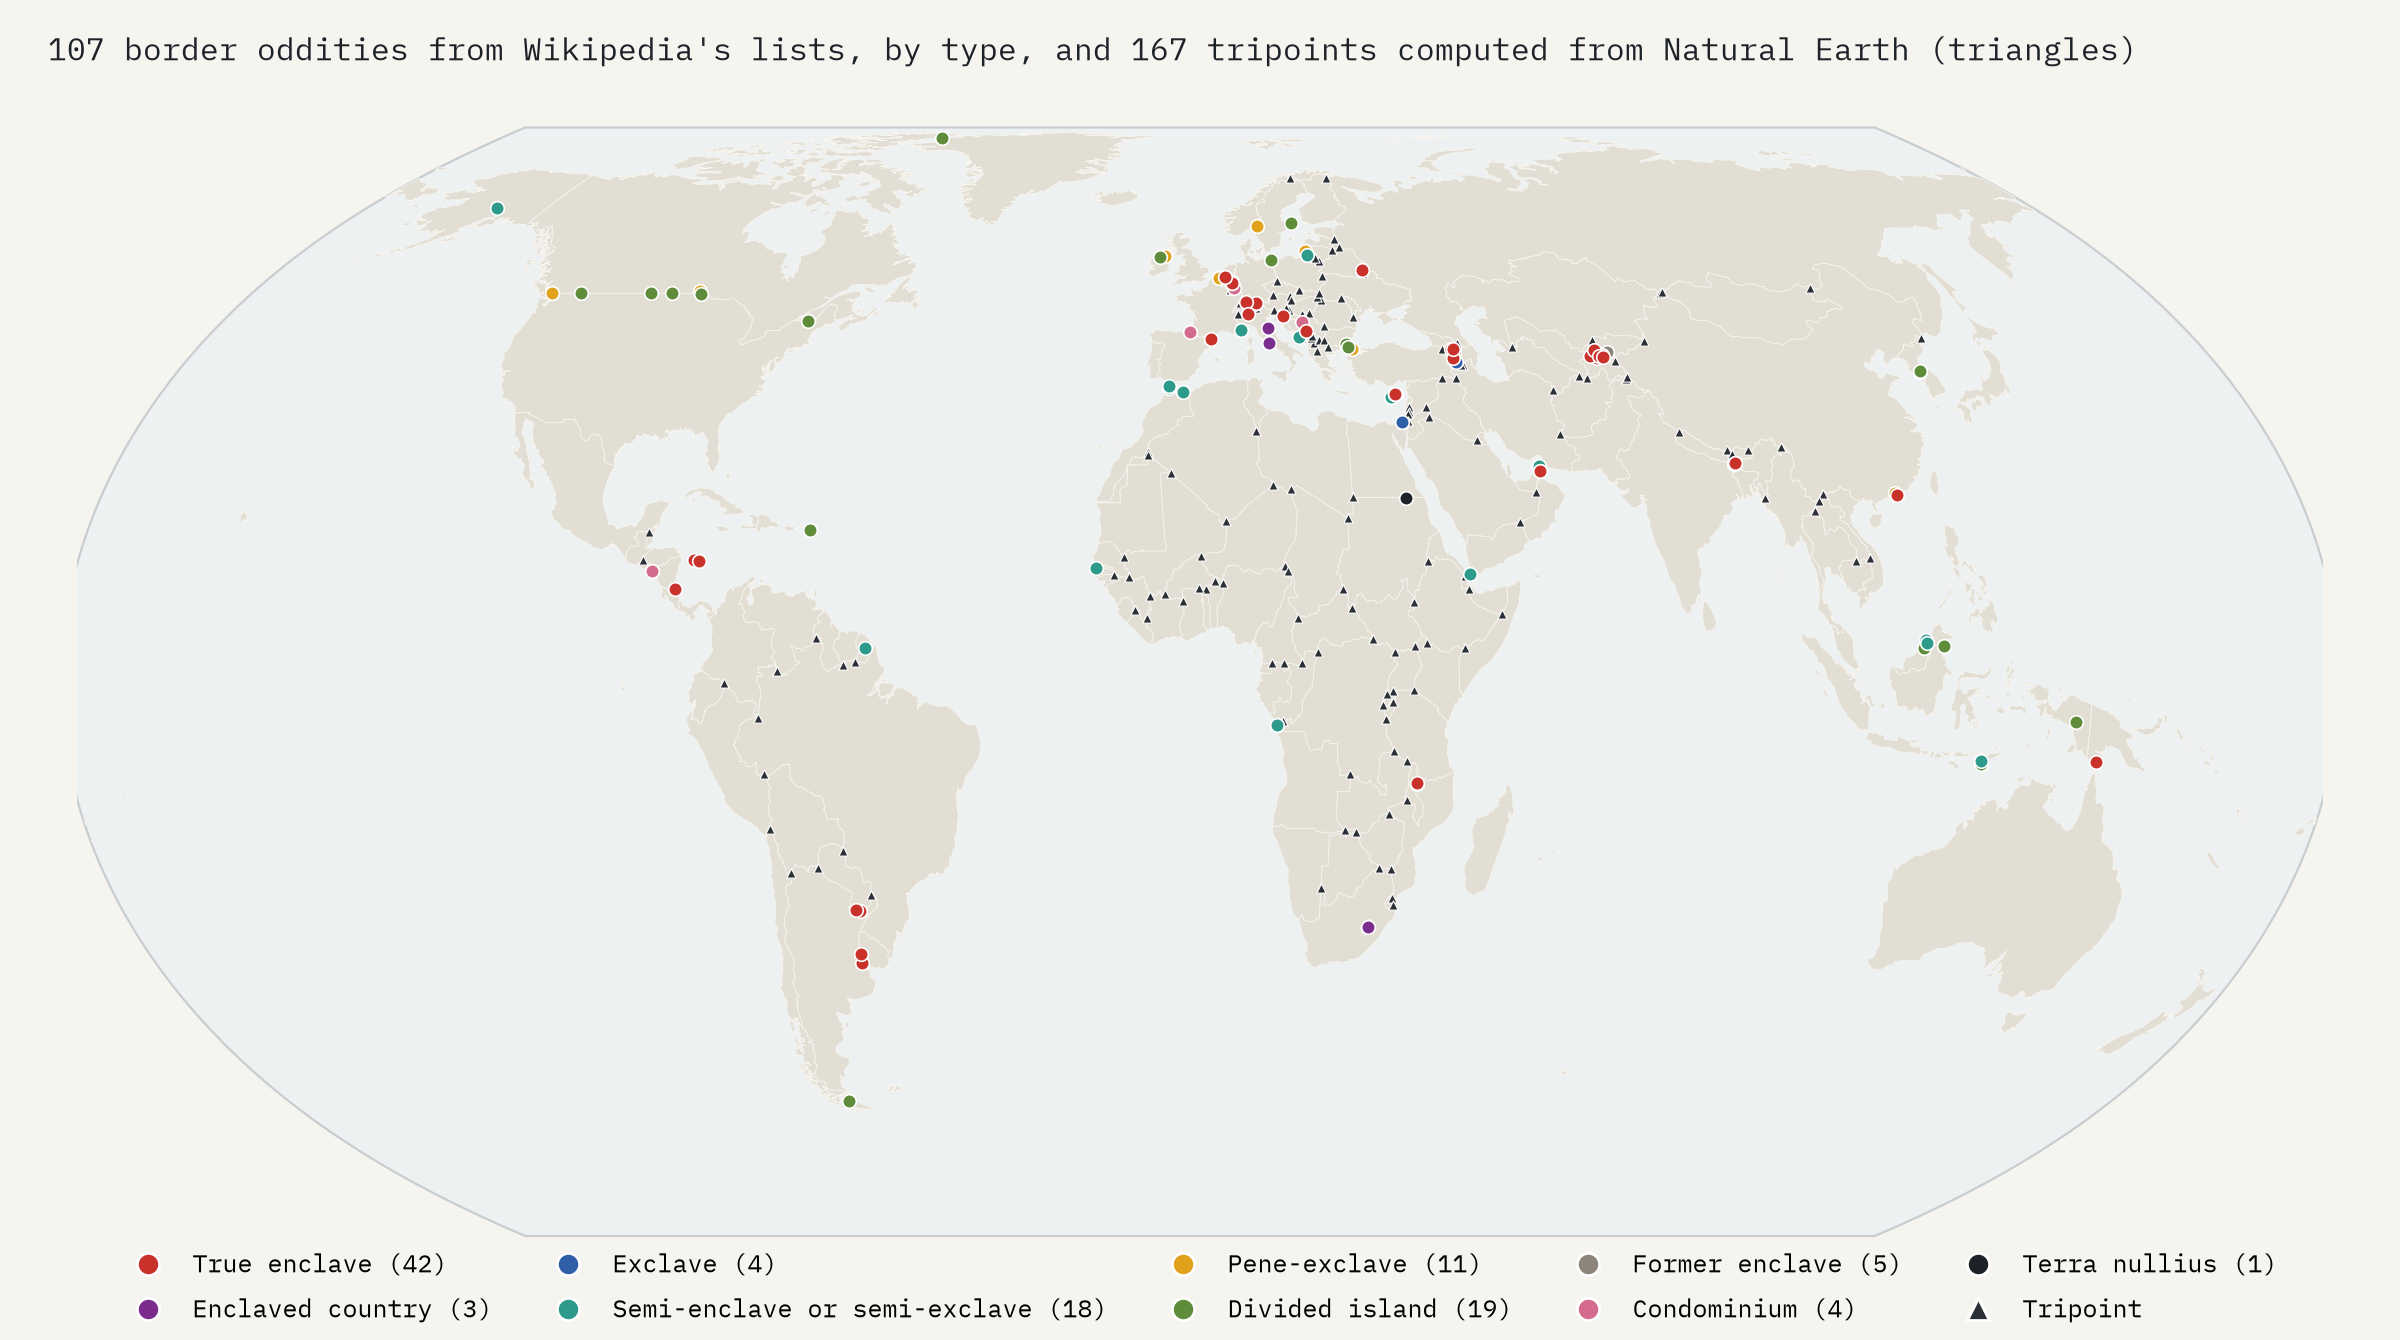
\includegraphics[width=\textwidth]{f_map.png}
\caption{The mapped catalogue by type, with tripoints computed from Natural Earth.}\label{fig:map}\end{figure}

Germany owns the most true enclaves (6): Büsingen and 5 pieces left west of the Vennbahn railway, whose trackbed the Treaty of Versailles gave to Belgium \citep{wvenn}. Belgium owns the most pieces, 22, all at Baarle. The largest true enclave on land is Uzbekistan's Sokh in Kyrgyzstan (234 km²) and the largest in water Argentina's Apipé islands (320 km²); the smallest entry is Germany's Rückschlag, 16,000 m², a house and garden. Among the enclaved countries Lesotho (30,355 km²) is the largest and the Vatican (0.44 km²) the smallest. Figure~\ref{fig:sizes} plots every area in the sources: from Baarle's parcel H7 (2,469 m²) to Lesotho is a factor of more than ten million.

\begin{figure}[tbp]\centering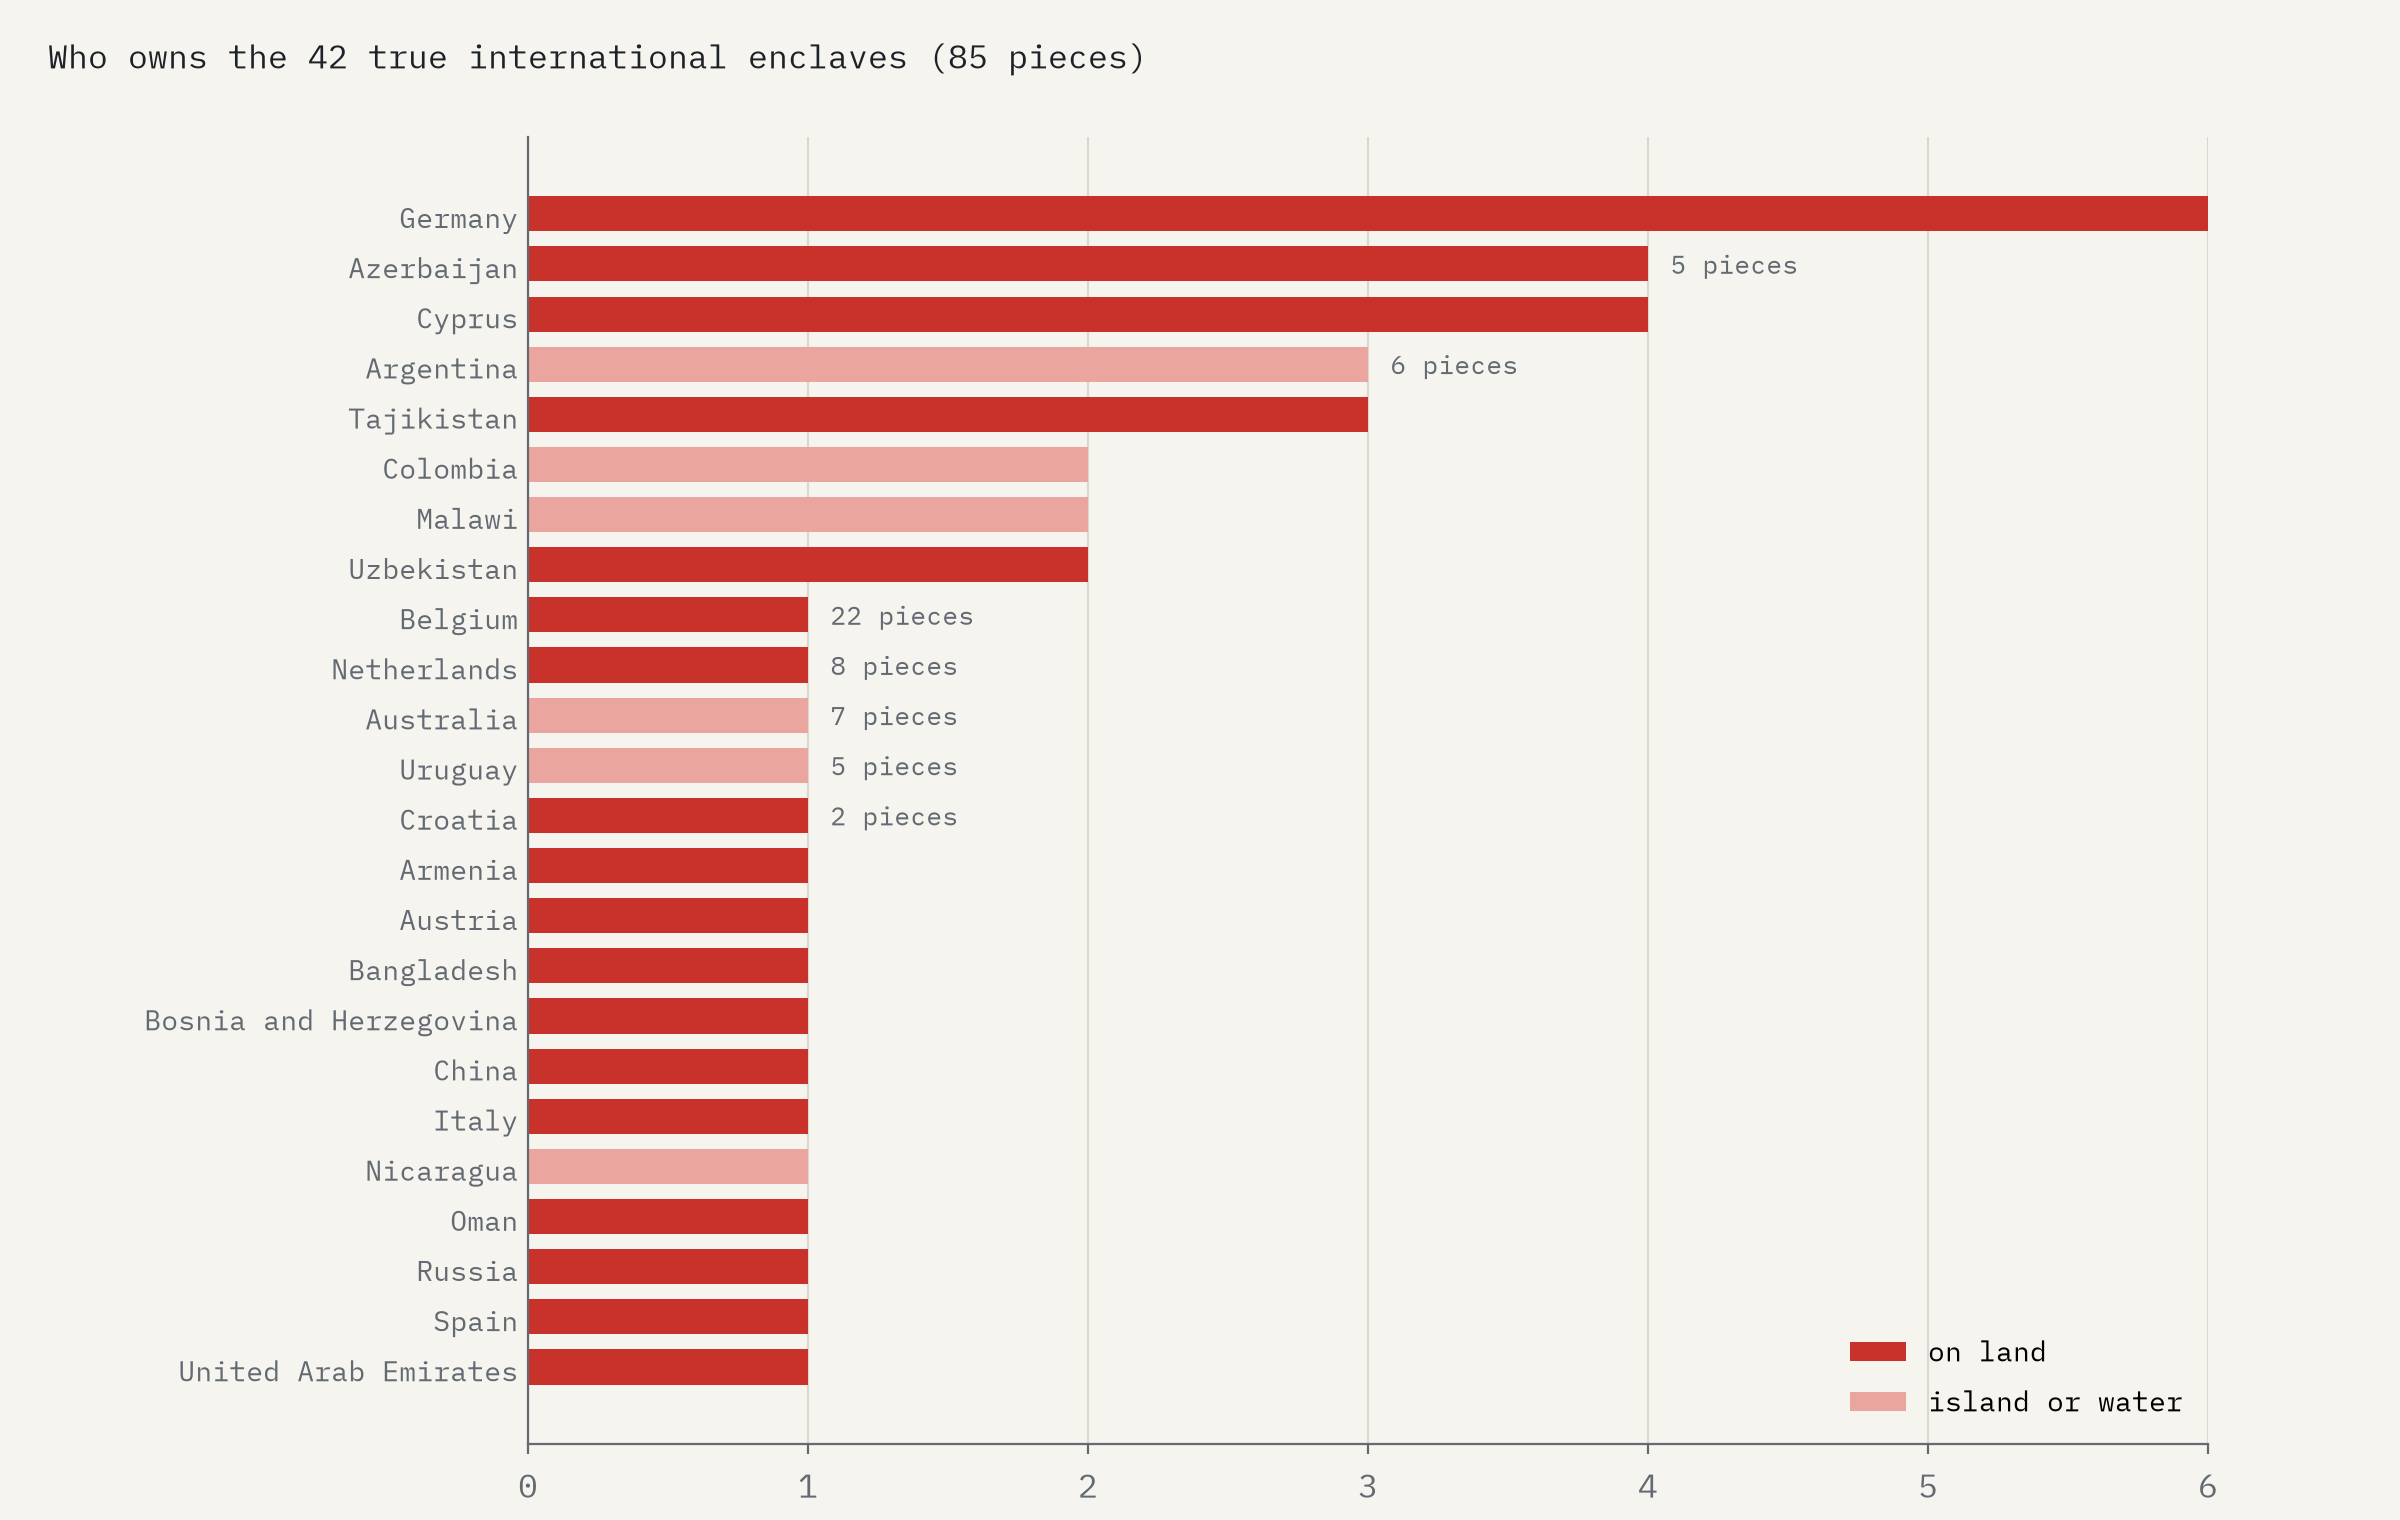
\includegraphics[width=\textwidth]{f_owners.png}
\caption{True international enclaves by owner, from Wikipedia's national-level table; labels give the number of separate pieces where it differs from the number of entries.}\label{fig:owners}\end{figure}

\begin{figure}[tbp]\centering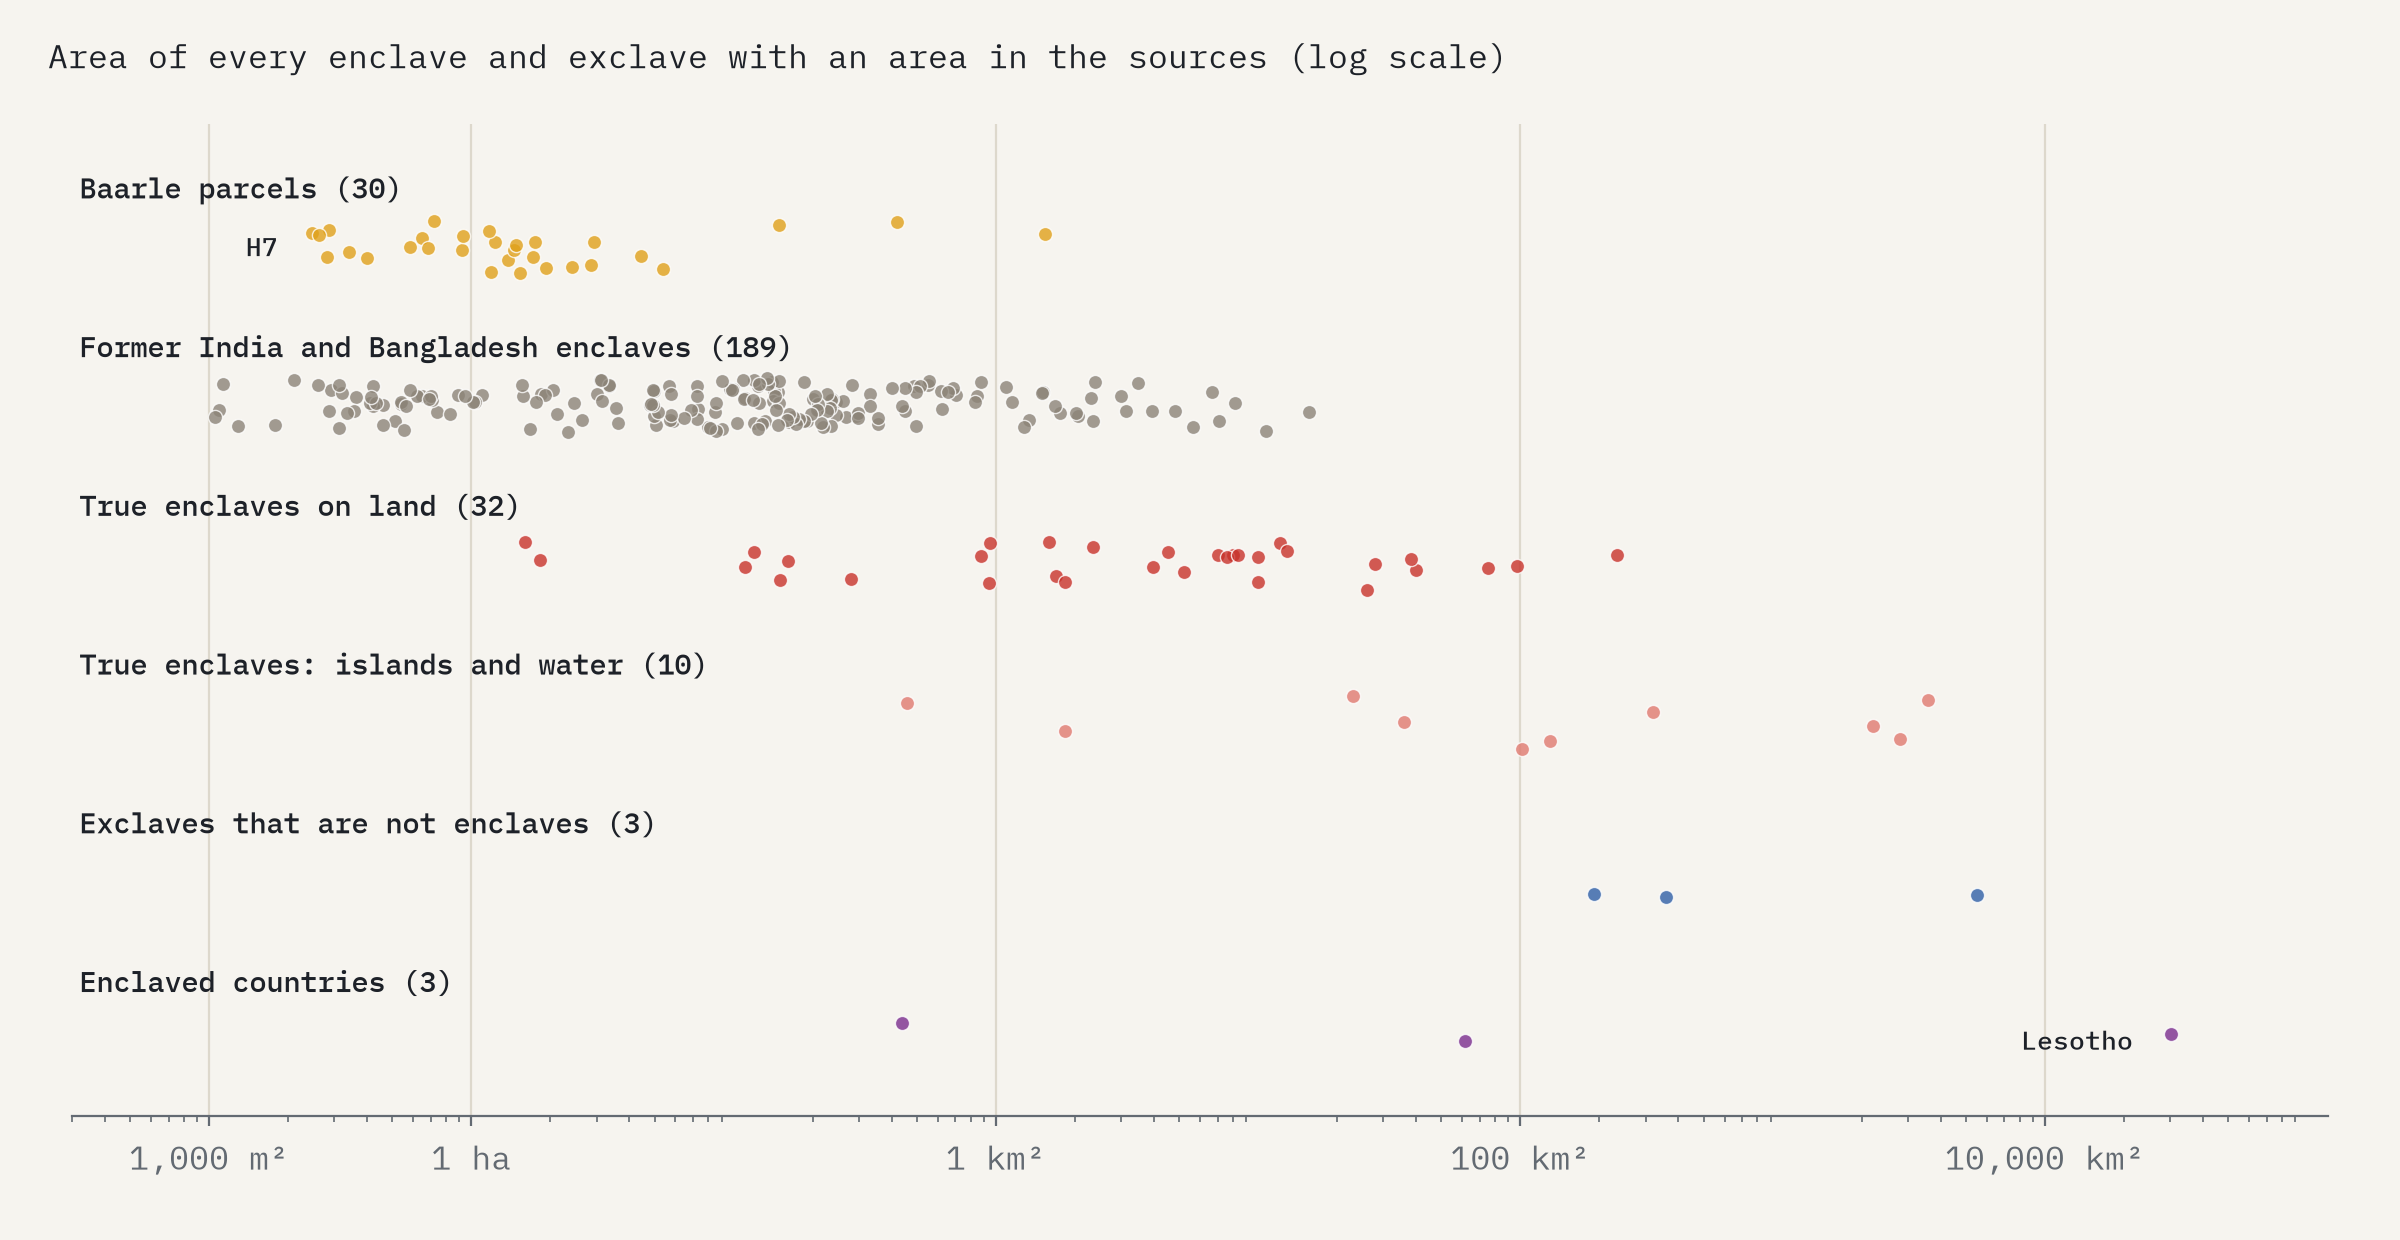
\includegraphics[width=\textwidth]{f_sizes.png}
\caption{Areas of enclaves and exclaves in the sources, on a log scale.}\label{fig:sizes}\end{figure}

\begin{longtable}{p{4.0cm}p{2.7cm}p{2.9cm}rrr}\caption{True international enclaves in Wikipedia's national-level list: owner, surrounding country, area (km², as listed), number of separate pieces, and whether Natural Earth 1:10m draws a separate piece within 3 km.}\label{tab:enclaves}\\\toprule Enclave & Belongs to & Inside & km² & Pieces & In NE\\\midrule\endfirsthead
\toprule Enclave & Belongs to & Inside & km² & Pieces & In NE\\\midrule\endhead
Apipé Islands & Argentina & Paraguay & 320 & 4 & \\
Isla Entre Ríos & Argentina & Paraguay & 36.0 & 1 & \\
Isla Martín García & Argentina & Uruguay & 1.8 & 1 & \\
Artsvashen & Armenia & Azerbaijan & 40.0 & 1 & yes\\
Torres Strait Islands & Australia & Papua New Guinea & 2,200 & 7 & \\
Jungholz & Austria & Germany & 7.0 & 1 & \\
Barkhudarli & Azerbaijan & Armenia & 10.0 & 1 & yes\\
Yukhari Askipara & Azerbaijan & Armenia & 28.0 & 1 & yes\\
Karki (Tigranashen) & Azerbaijan & Armenia & 8.0 & 1 & \\
Yaradullu & Azerbaijan & Armenia & 0.120 & 2 & \\
Dahagram-Angarpota & Bangladesh & India & 25.9 & 1 & \\
Baarle-Hertog & Belgium & Netherlands & 2.3 & 22 & \\
Međurečje & Bosnia and Herzegovina & Serbia & 4.0 & 1 & \\
West Kowloon Port & China & Hong Kong & 0.110 & 1 & \\
Quitasueño & Colombia & Nicaragua & 3,577 & 1 & \\
Serrana & Colombia & Nicaragua & 2,800 & 1 & \\
Brezovica Žumberačka & Croatia & Slovenia & 0.018 & 2 & \\
Ormidhia & Cyprus & Dhekelia Sovereign Base Area & 1.7 & 1 & yes\\
Xylotymbou & Cyprus & Dhekelia Sovereign Base Area & 0.947 & 1 & yes\\
Electricity Authority refugee settlement & Cyprus & Dhekelia Sovereign Base Area & 0.280 & 1 & yes\\
Dhekelia Power Station & Cyprus & Dhekelia Sovereign Base Area & 0.161 & 1 & yes\\
Münsterbildchen & Germany & Belgium & 1.8 & 1 & \\
Roetgener Wald & Germany & Belgium & 10.0 & 1 & \\
Rückschlag & Germany & Belgium & 0.016 & 1 & \\
Mützenich & Germany & Belgium & 12.1 & 1 & \\
Ruitzhof & Germany & Belgium & 0.937 & 1 & \\
Büsingen am Hochrhein & Germany & Switzerland & 7.6 & 1 & \\
Campione d'Italia & Italy & Switzerland & 1.6 & 1 & \\
Likoma Island & Malawi & Mozambique & 130 & 1 & yes\\
Chizumulu Island & Malawi & Mozambique & 101 & 1 & yes\\
Baarle-Nassau & Netherlands & Belgium & 0.151 & 8 & \\
Laguna Los Portillos & Nicaragua & Costa Rica & 0.460 & 1 & yes\\
Madha & Oman & United Arab Emirates & 75.0 & 1 & yes\\
Sankovo-Medvezhye & Russia & Belarus & 4.5 & 1 & \\
Llívia & Spain & France & 12.8 & 1 & yes\\
Vorukh & Tajikistan & Kyrgyzstan & 96.7 & 1 & yes\\
Lolazor & Tajikistan & Kyrgyzstan & 0.880 & 1 & \\
Sarvan & Tajikistan & Uzbekistan & 8.4 & 1 & yes\\
Nahwa & United Arab Emirates & Oman & 5.2 & 1 & yes\\
Filomena Islands & Uruguay & Argentina & 23.0 & 5 & \\
Sokh & Uzbekistan & Kyrgyzstan & 234 & 1 & yes\\
Shakhimardan & Uzbekistan & Kyrgyzstan & 38.2 & 1 & yes\\
\bottomrule\end{longtable}

\subsection{Nested enclaves}
Baarle's parcel tables list 22 Belgian exclaves in the Netherlands, from H1 (153.6 ha) to H7 (2,469 m²), and 8 Dutch parcels, seven of them counter-enclaves inside Belgian exclaves (Figure~\ref{fig:baarle}) \citep{wbh,wbn}. The tables have the boundary running through about 54 homes; in H7 it divides a front door, which has a Belgian and a Dutch house number. Along the India and Bangladesh border there were 102 Indian enclaves in Bangladesh, containing 21 Bangladeshi counter-enclaves, and 71 Bangladeshi enclaves in India, containing 3 Indian counter-enclaves, one of which contained the only third-order enclave, Dahala Khagrabari (6,880 m²) \citep{wib}. A joint census in 2010 counted 51,549 residents. The enclaves were exchanged at midnight on 31 July 2015: Bangladesh received 111 and India 51; Dahagram-Angarpota alone remains, linked to Bangladesh by the Tin Bigha Corridor \citep{wdahagram}. The only nested pair now at national level is Madha, a piece of Oman in the United Arab Emirates, and Nahwa, a piece of Sharjah inside Madha \citep{wmadha,wnahwa}.

\begin{figure}[tbp]\centering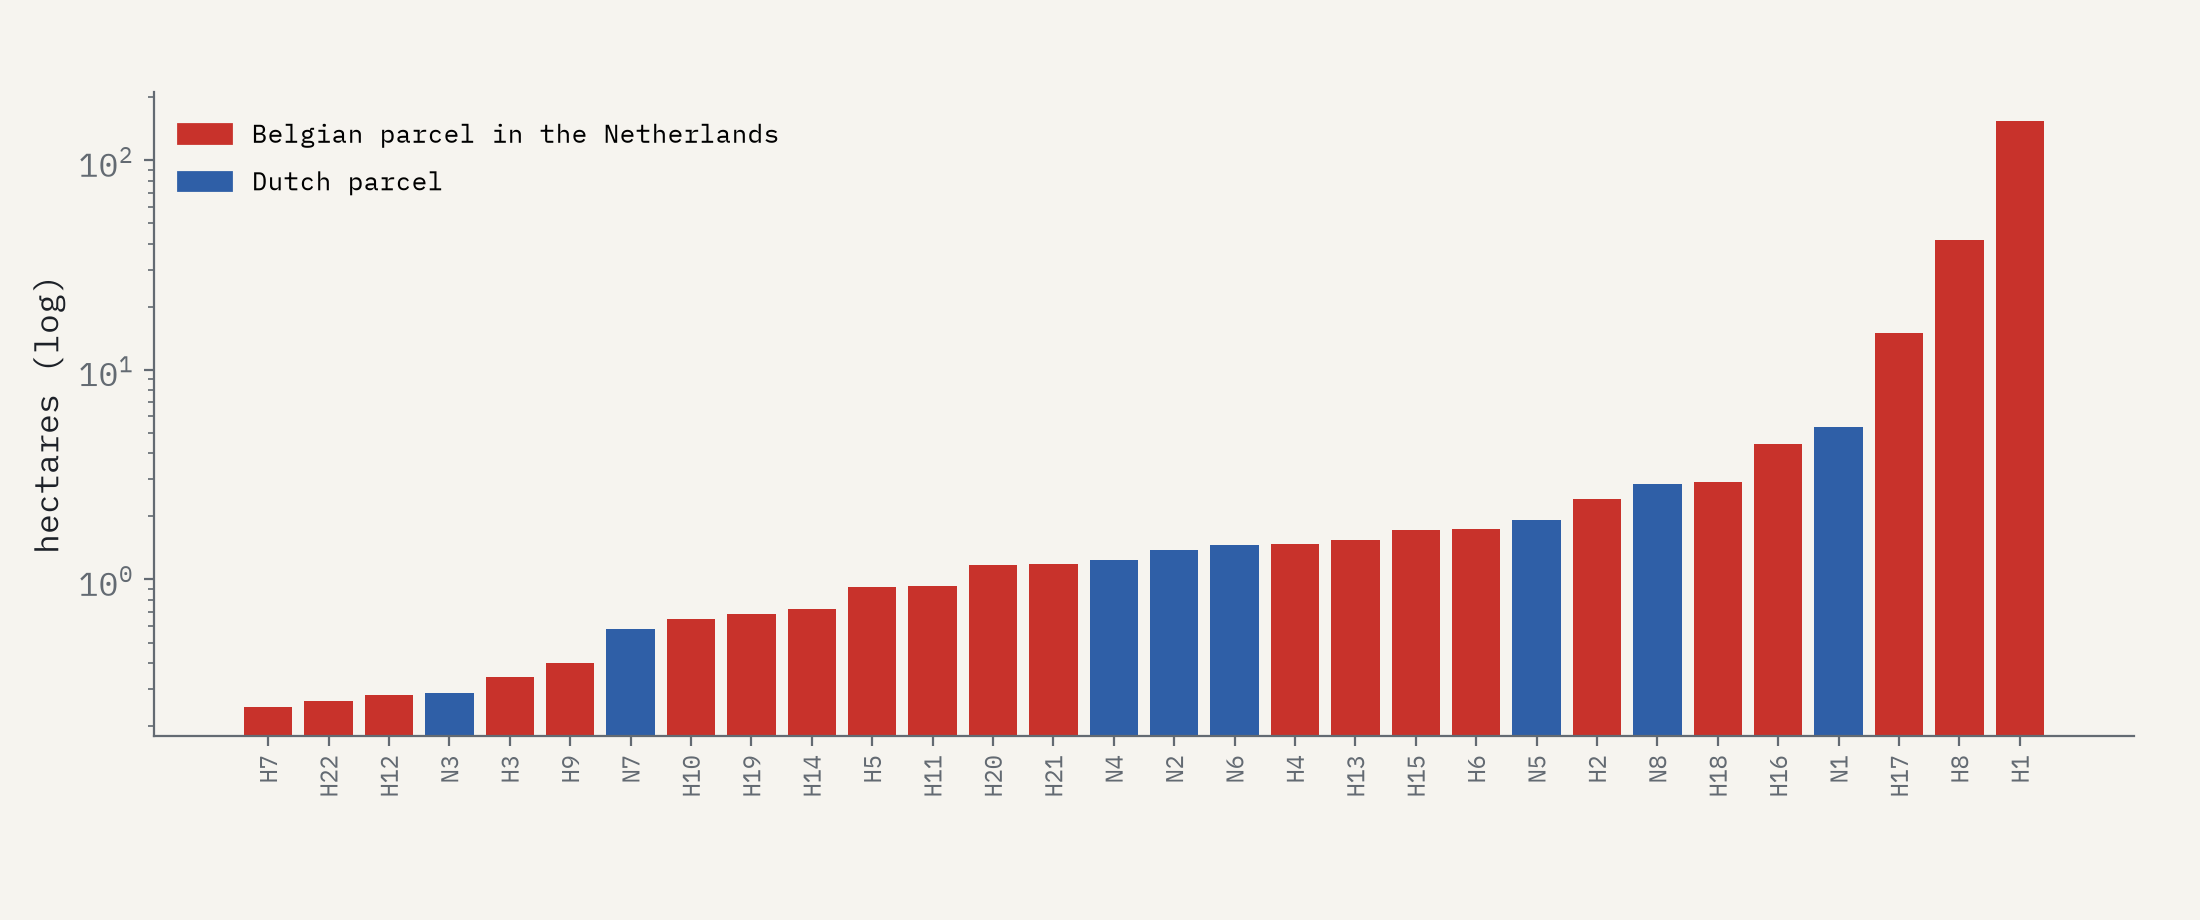
\includegraphics[width=\textwidth]{f_baarle.png}
\caption{Baarle's 30 parcels by area (log scale), from Wikipedia's parcel tables.}\label{fig:baarle}\end{figure}

\subsection{Tripoints and the quadripoint}
Natural Earth yields 167 tripoints between three countries, one point where four meet, and 14 more points where two countries meet an indeterminate zone. Wikipedia's tripoint article gave 181 international tripoints in 2020 and its list has 176 rows, including de facto states that Natural Earth does not separate \citep{wtri,wtrilist}. China has the most (15; Wikipedia's list, 16), then Russia (10; 13). 26 countries with land neighbours have no tripoint. Natural Earth's single quadripoint is at Kazungula, between Botswana, Namibia, Zambia and Zimbabwe; Wikipedia reports that all four states agreed in the late 2000s that Botswana and Zambia share a border of about 150 m, so there are two tripoints about 100 to 150 m apart \citep{wquad}. At 1:10m the gap is not drawn.

\subsection{Neighbours, borders and landlocked countries}
China and Russia each have 14 neighbours, France 11 (through French Guiana and Saint-Martin) and Brazil 10 (Figure~\ref{fig:nei}). Natural Earth and Wikipedia's land border table \citep{wland} agree on the number of neighbours for 150 of the 160 countries found in both. The 10 differences arise from borders too short to draw (Botswana and Zambia; Bahrain and Saudi Arabia on the King Fahd Causeway), from Hans Island, split between Canada and Denmark in 2022 \citep{whans}, from Natural Earth's de facto lines (Kashmir, Somaliland) and from counting dependencies with their sovereign. 18 countries have one neighbour in Natural Earth. The longest border between two countries is Canada and the United States (7,936 km), then Kazakhstan and Russia (6,658 km). Russia's land borders total 19,013 km and China's 18,995 km in Natural Earth, against 20,017 km and 22,147 km in Wikipedia's table: generalisation shortens lines, and shrinks the border of Italy and the Vatican to 430 m.

With the Caspian as a lake, 45 countries are landlocked, exactly Wikipedia's 44 sovereign landlocked countries plus Kosovo \citep{wlandlocked}. Liechtenstein (between Austria and Switzerland) and Uzbekistan (between Afghanistan, Kazakhstan, Kyrgyzstan, Tajikistan and Turkmenistan) are doubly landlocked (Figure~\ref{fig:landlocked}); Uzbekistan's status depends on treating the Caspian as a lake.

\begin{figure}[tbp]\centering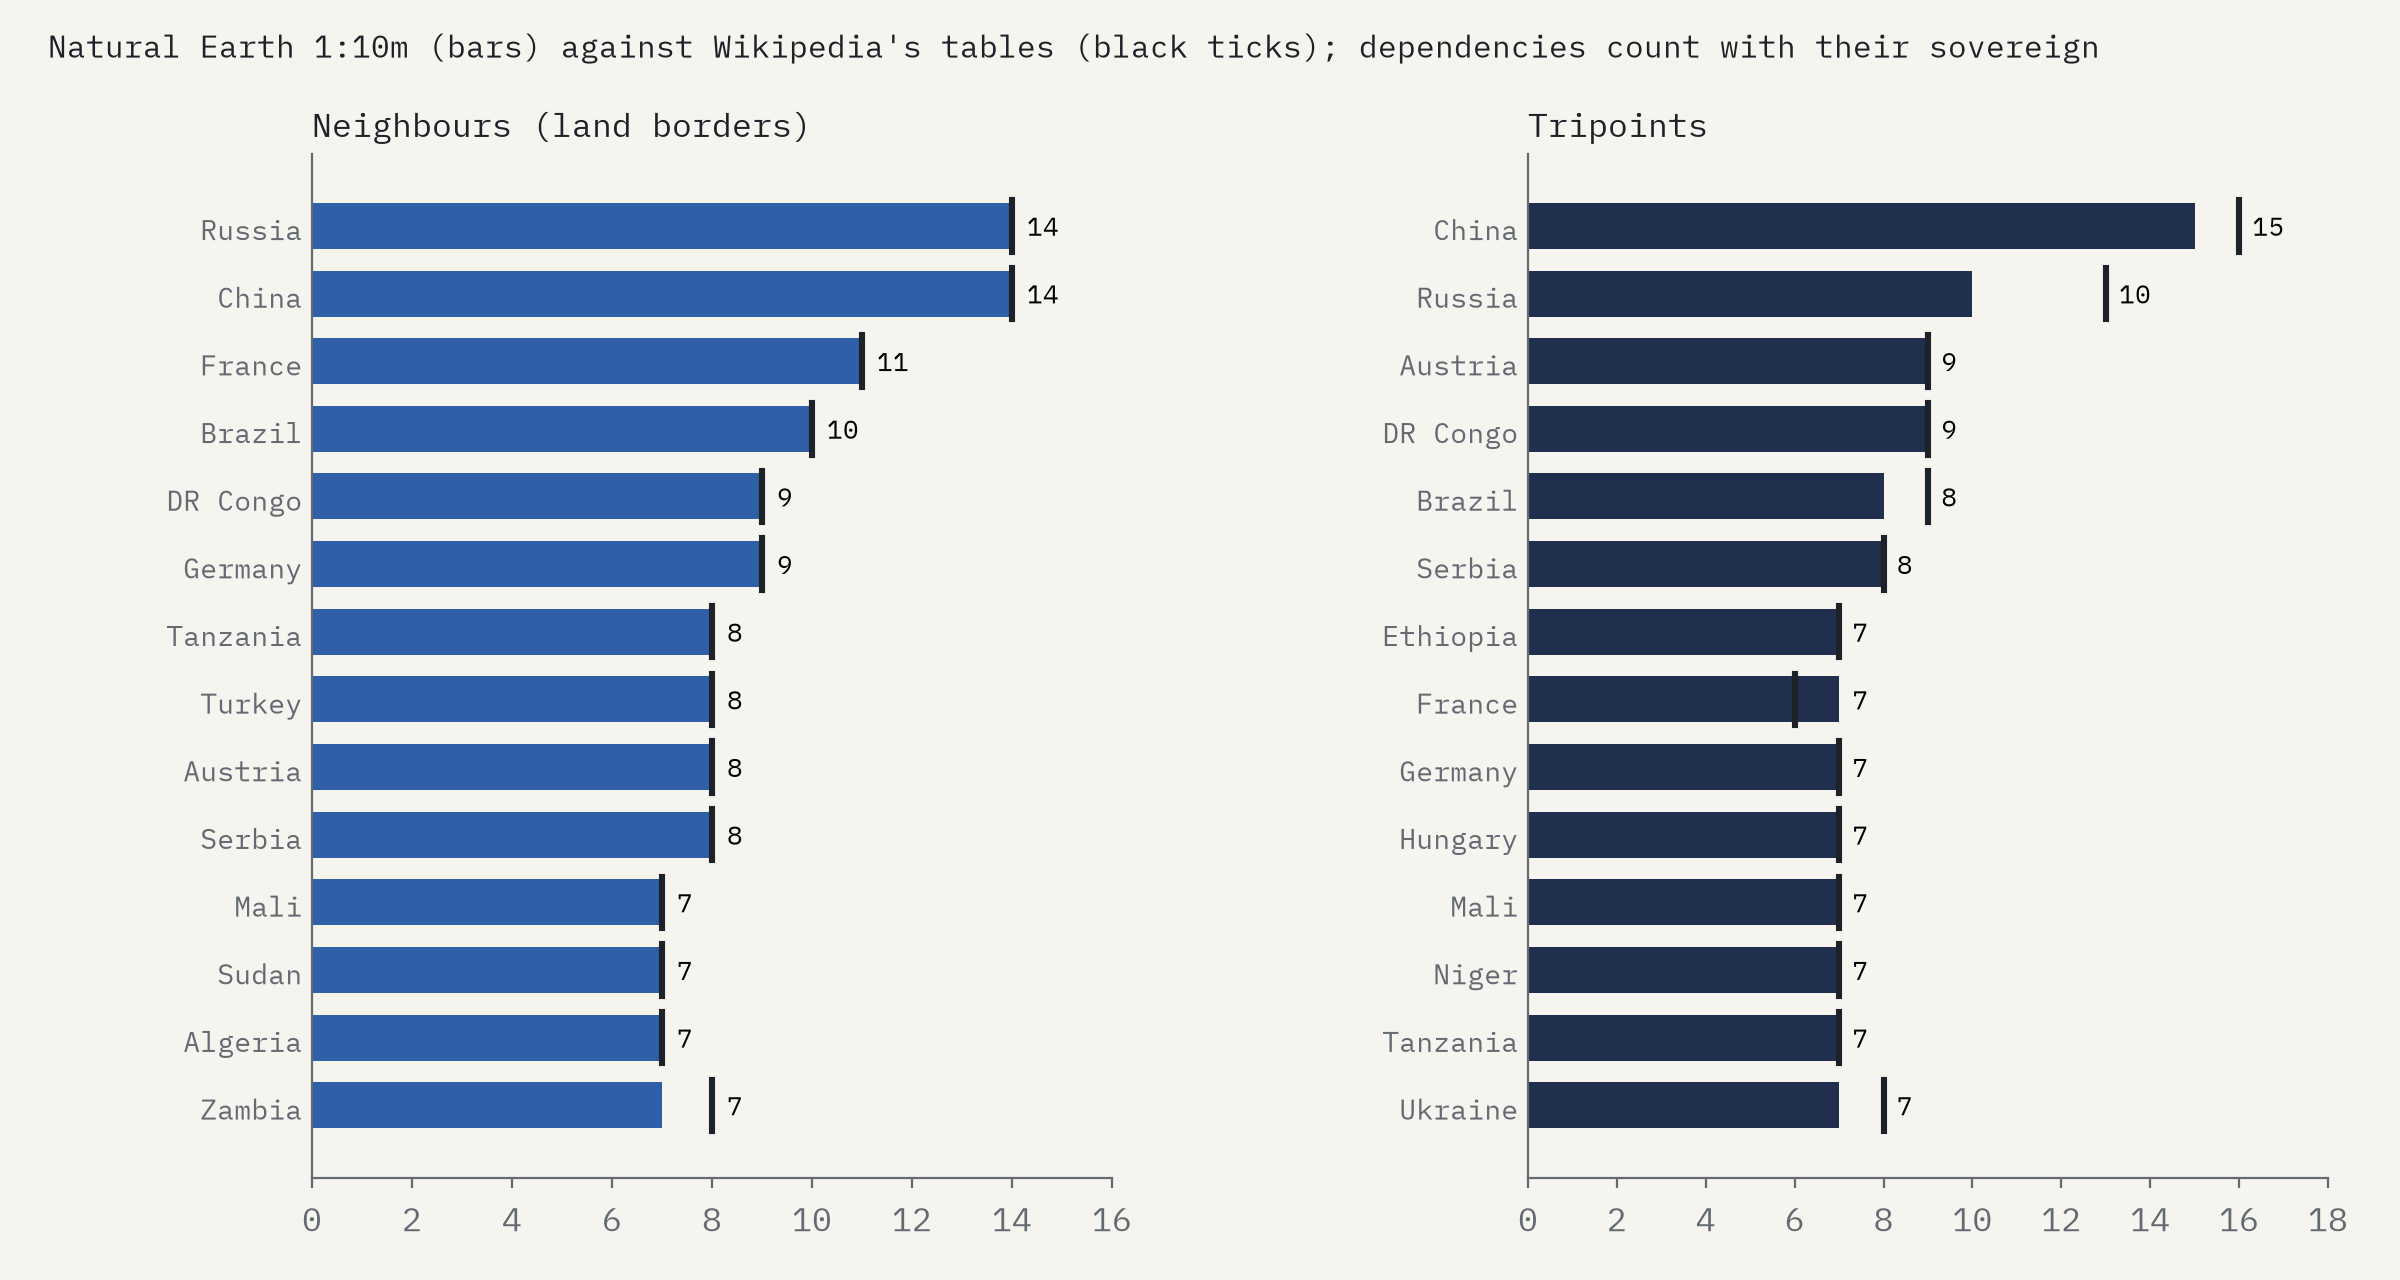
\includegraphics[width=\textwidth]{f_neighbours.png}
\caption{Neighbours and tripoints per country in Natural Earth (bars) and Wikipedia (ticks).}\label{fig:nei}\end{figure}

\begin{figure}[tbp]\centering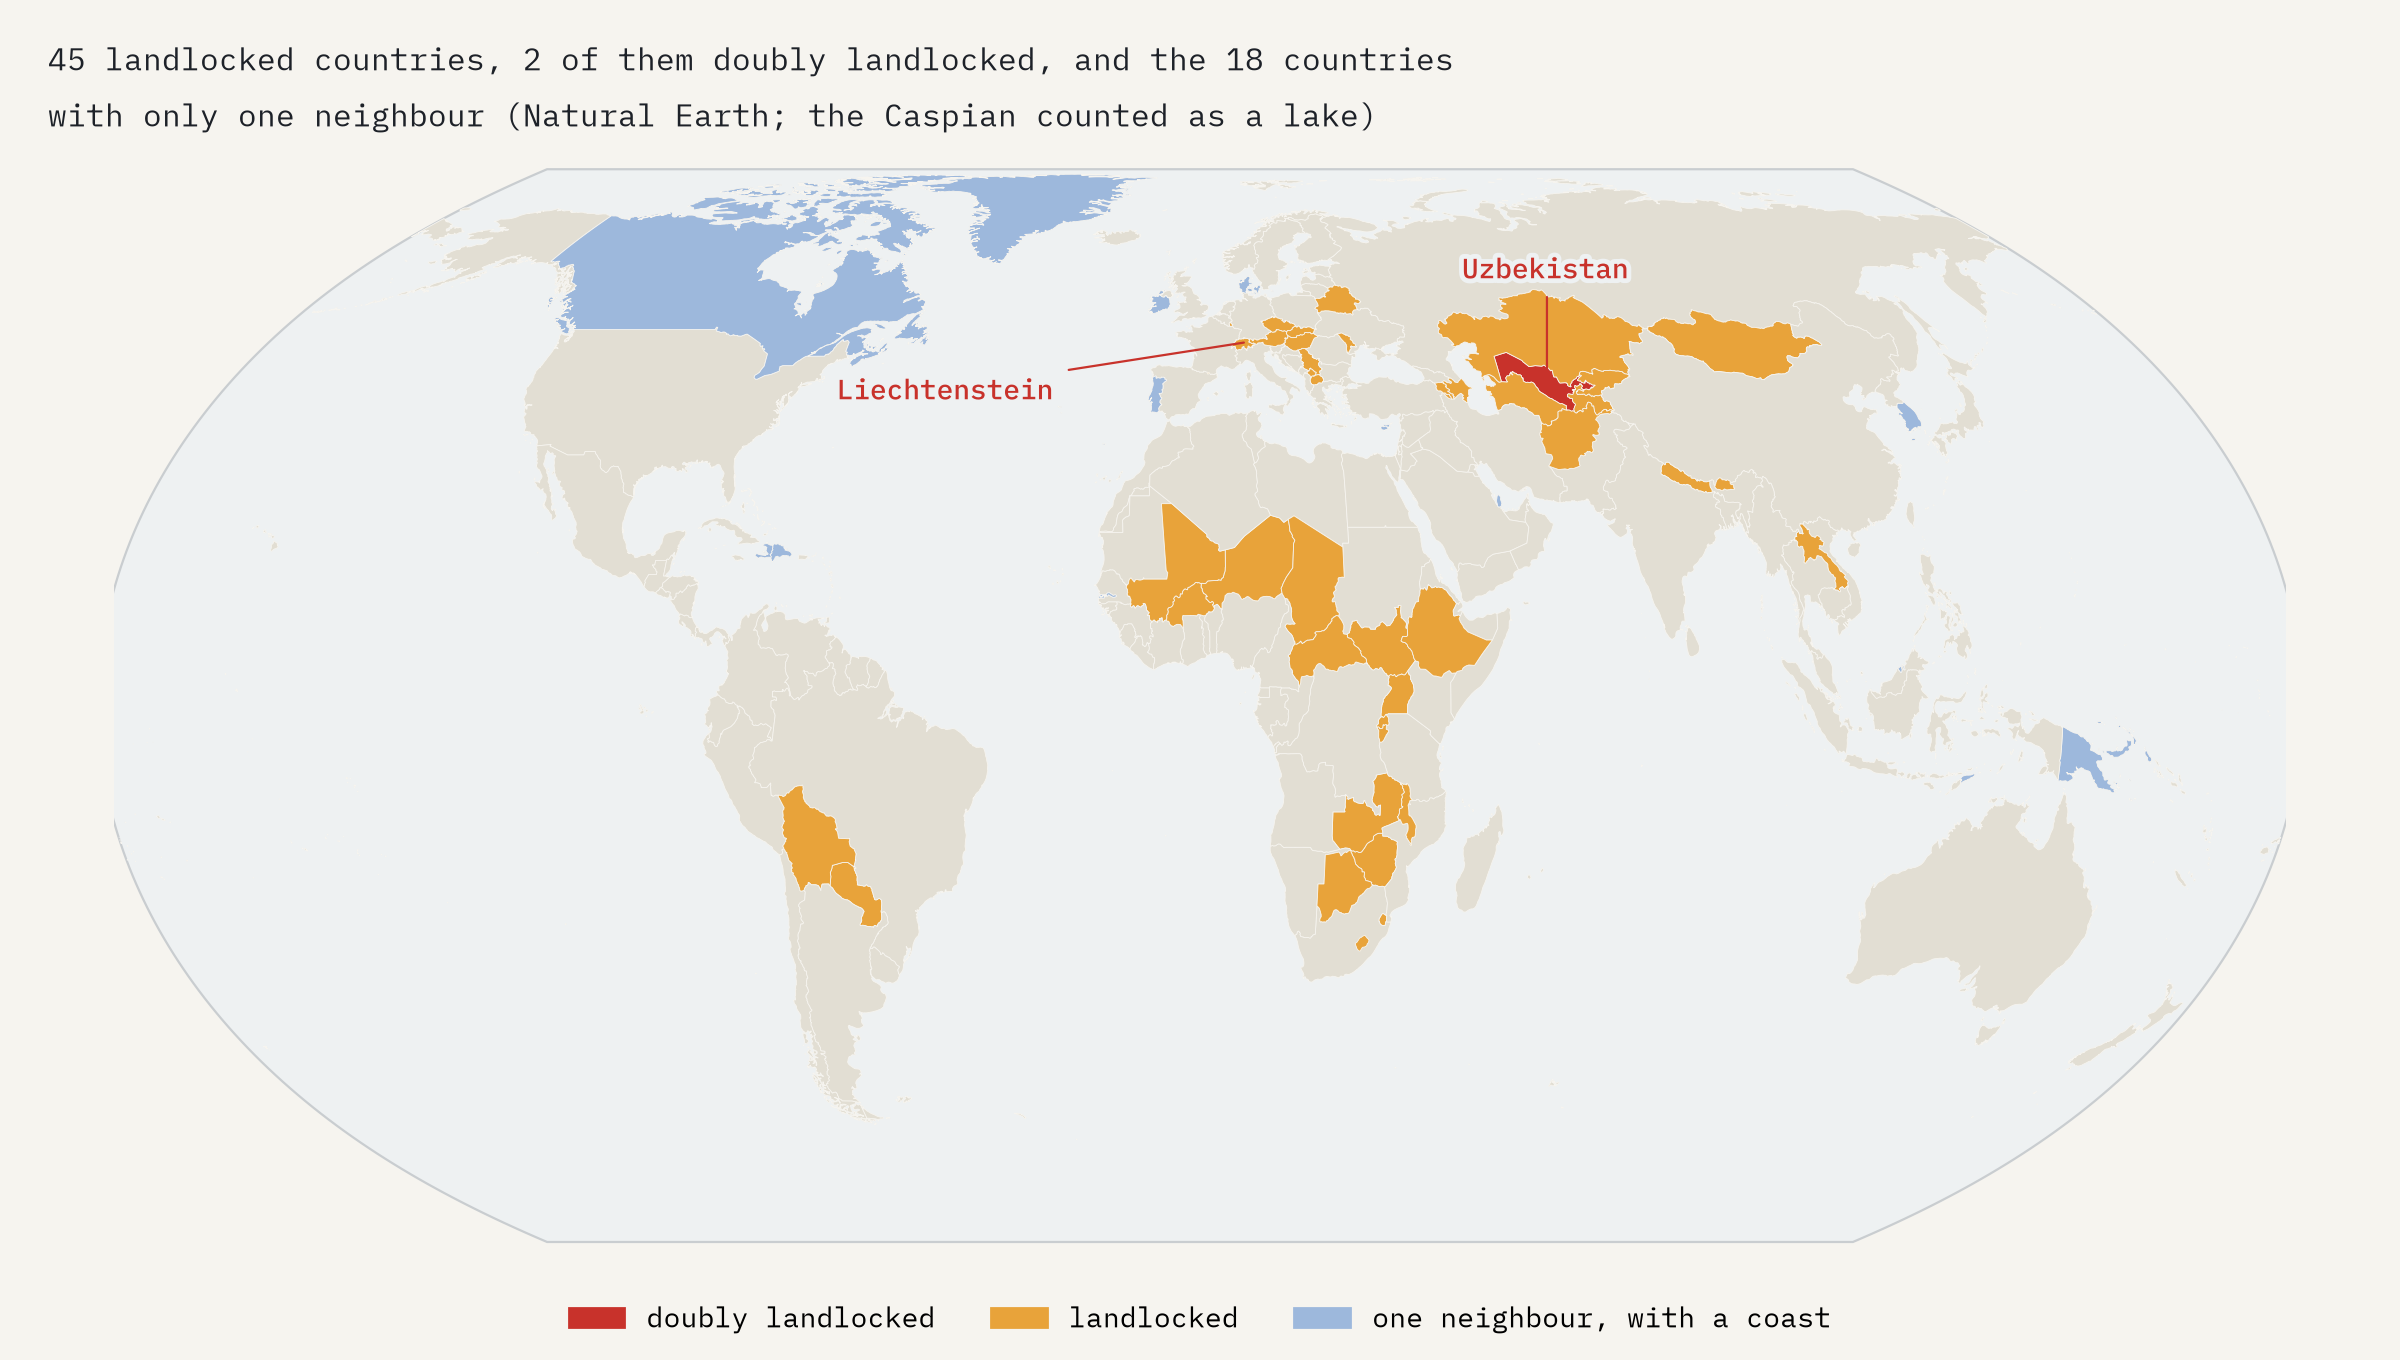
\includegraphics[width=\textwidth]{f_landlocked.png}
\caption{Landlocked and doubly landlocked countries, and countries with one neighbour, in Natural Earth.}\label{fig:landlocked}\end{figure}

\subsection{What Natural Earth contains}
Natural Earth contains 50 detached pieces that touch another country: 13 enclaves, 1 landlocked exclave (Nakhchivan), 19 coastal exclaves and 17 pieces of shared islands (Table~\ref{tab:ne}). The United Kingdom has the most (4). The largest is Alaska (1,427,512 km²) and the smallest a lagoon of Nicaragua's on the Costa Rican coast (1.19 km²). Two are artefacts of drawing rather than oddities of sovereignty: Canada south and east of the St Lawrence, separated because the river is drawn as water, and Crimea, which Natural Earth's de facto line shows with Russia. Of Wikipedia's 42 true enclaves, 17 are drawn as separate pieces; Baarle, Büsingen, Campione and Jungholz are absent. Figure~\ref{fig:insets} shows the tour's 15 places as Natural Earth draws them.

{\footnotesize\begin{longtable}{p{2.6cm}p{4.4cm}p{2.6cm}rp{3.4cm}}\caption{Detached pieces of countries that touch another country in Natural Earth 1:10m, named after the catalogue entry they contain where there is one.}\label{tab:ne}\\\toprule Country & Place & Type & km² & Touches\\\midrule\endfirsthead
\toprule Country & Place & Type & km² & Touches\\\midrule\endhead
United States & Alaska & coastal exclave & 1,427,512.4 & Canada\\
Indonesia & New Guinea & part of a shared island & 381,927.2 & Papua New Guinea\\
Canada & Canada south and east of the St Lawrence (river drawn as water) & coastal exclave & 203,081.4 & United States\\
Malaysia & Borneo & part of a shared island & 194,965.2 & Brunei; Indonesia\\
France & French Guiana & coastal exclave & 83,183.7 & Brazil; Suriname\\
Russia & Crimea (Natural Earth's de facto line) & coastal exclave & 27,096.0 & Ukraine\\
Chile & Tierra del Fuego & part of a shared island & 26,555.8 & Argentina\\
Turkey & East Thrace (Turkey in Europe) & coastal exclave & 23,386.9 & Bulgaria; Greece\\
Argentina & Tierra del Fuego (Argentina) & part of a shared island & 20,551.7 & Chile\\
United Kingdom & Northern Ireland & part of a shared island & 14,238.8 & Ireland\\
Indonesia & Timor & part of a shared island & 13,830.1 & Timor-Leste\\
Russia & Kaliningrad & coastal exclave & 13,449.4 & Lithuania; Poland\\
Angola & Cabinda & coastal exclave & 6,701.7 & DR Congo; Republic of the Congo\\
Azerbaijan & Nakhchivan & landlocked exclave & 4,782.9 & Armenia; Iran; Turkey\\
Oman & Musandam & coastal exclave & 1,579.3 & United Arab Emirates\\
Brunei & Temburong & part of a shared island & 1,298.9 & Malaysia\\
Netherlands & Zeelandic Flanders & coastal exclave & 824.6 & Belgium\\
Croatia & Dubrovnik and southern Dalmatia & coastal exclave & 750.1 & Bosnia and Herzegovina; Montenegro\\
Timor-Leste & Oecusse & part of a shared island & 739.4 & Indonesia\\
Uzbekistan & Sokh & enclave & 399.4 & Kyrgyzstan\\
Germany & Usedom (Germany) & coastal exclave & 374.7 & Poland\\
Palestine & Gaza Strip & coastal exclave & 339.4 & Egypt; Israel\\
Malaysia & Sebatik & part of a shared island & 212.4 & Indonesia\\
Indonesia & Sebatik (Indonesia) & part of a shared island & 212.3 & Malaysia\\
Cyprus & Famagusta and eastern Larnaca (Cyprus) & part of a shared island & 193.6 & United Kingdom\\
Lithuania & Curonian Spit (Lithuania) & coastal exclave & 133.2 & Russia\\
United Kingdom & Dhekelia & part of a shared island & 127.4 & Northern Cyprus; Cyprus\\
Tajikistan & Vorukh & enclave & 119.5 & Kyrgyzstan\\
Malawi & Likoma Island & enclave & 119.2 & Mozambique\\
United Kingdom & Akrotiri & part of a shared island & 98.7 & Cyprus\\
Oman & Madha & enclave & 98.2 & United Arab Emirates\\
Malawi & Chizumulu Island & enclave & 80.2 & Mozambique\\
France & Saint-Martin & part of a shared island & 68.3 & Netherlands\\
Ivory Coast &  & coastal exclave & 64.7 & Ghana\\
Uzbekistan & Shakhimardan & enclave & 58.3 & Kyrgyzstan\\
Spain & Ceuta & coastal exclave & 42.7 & Morocco\\
Armenia & Artsvashen & enclave & 35.2 & Azerbaijan\\
Tajikistan & Sarvan & enclave & 30.5 & Uzbekistan\\
Argentina &  & part of a shared island & 28.4 & Chile\\
Azerbaijan & Yukhari Askipara & enclave & 26.8 & Armenia\\
Netherlands & Sint Maarten & part of a shared island & 23.4 & France\\
Spain & Melilla & coastal exclave & 18.1 & Morocco\\
Spain & Llívia & enclave & 13.2 & France\\
Azerbaijan & Barkhudarli & enclave & 7.3 & Armenia\\
United Arab Emirates & Nahwa & enclave & 7.3 & Oman\\
United States & Point Roberts & coastal exclave & 5.4 & Canada\\
United Kingdom & Gibraltar & coastal exclave & 3.7 & Spain\\
Cyprus & Famagusta and eastern Larnaca (Cyprus) & part of a shared island & 2.1 & United Kingdom\\
Cyprus & Famagusta and eastern Larnaca (Cyprus) & enclave & 1.5 & United Kingdom\\
Nicaragua & Laguna Los Portillos & coastal exclave & 1.2 & Costa Rica\\
\bottomrule\end{longtable}}

\begin{figure}[tbp]\centering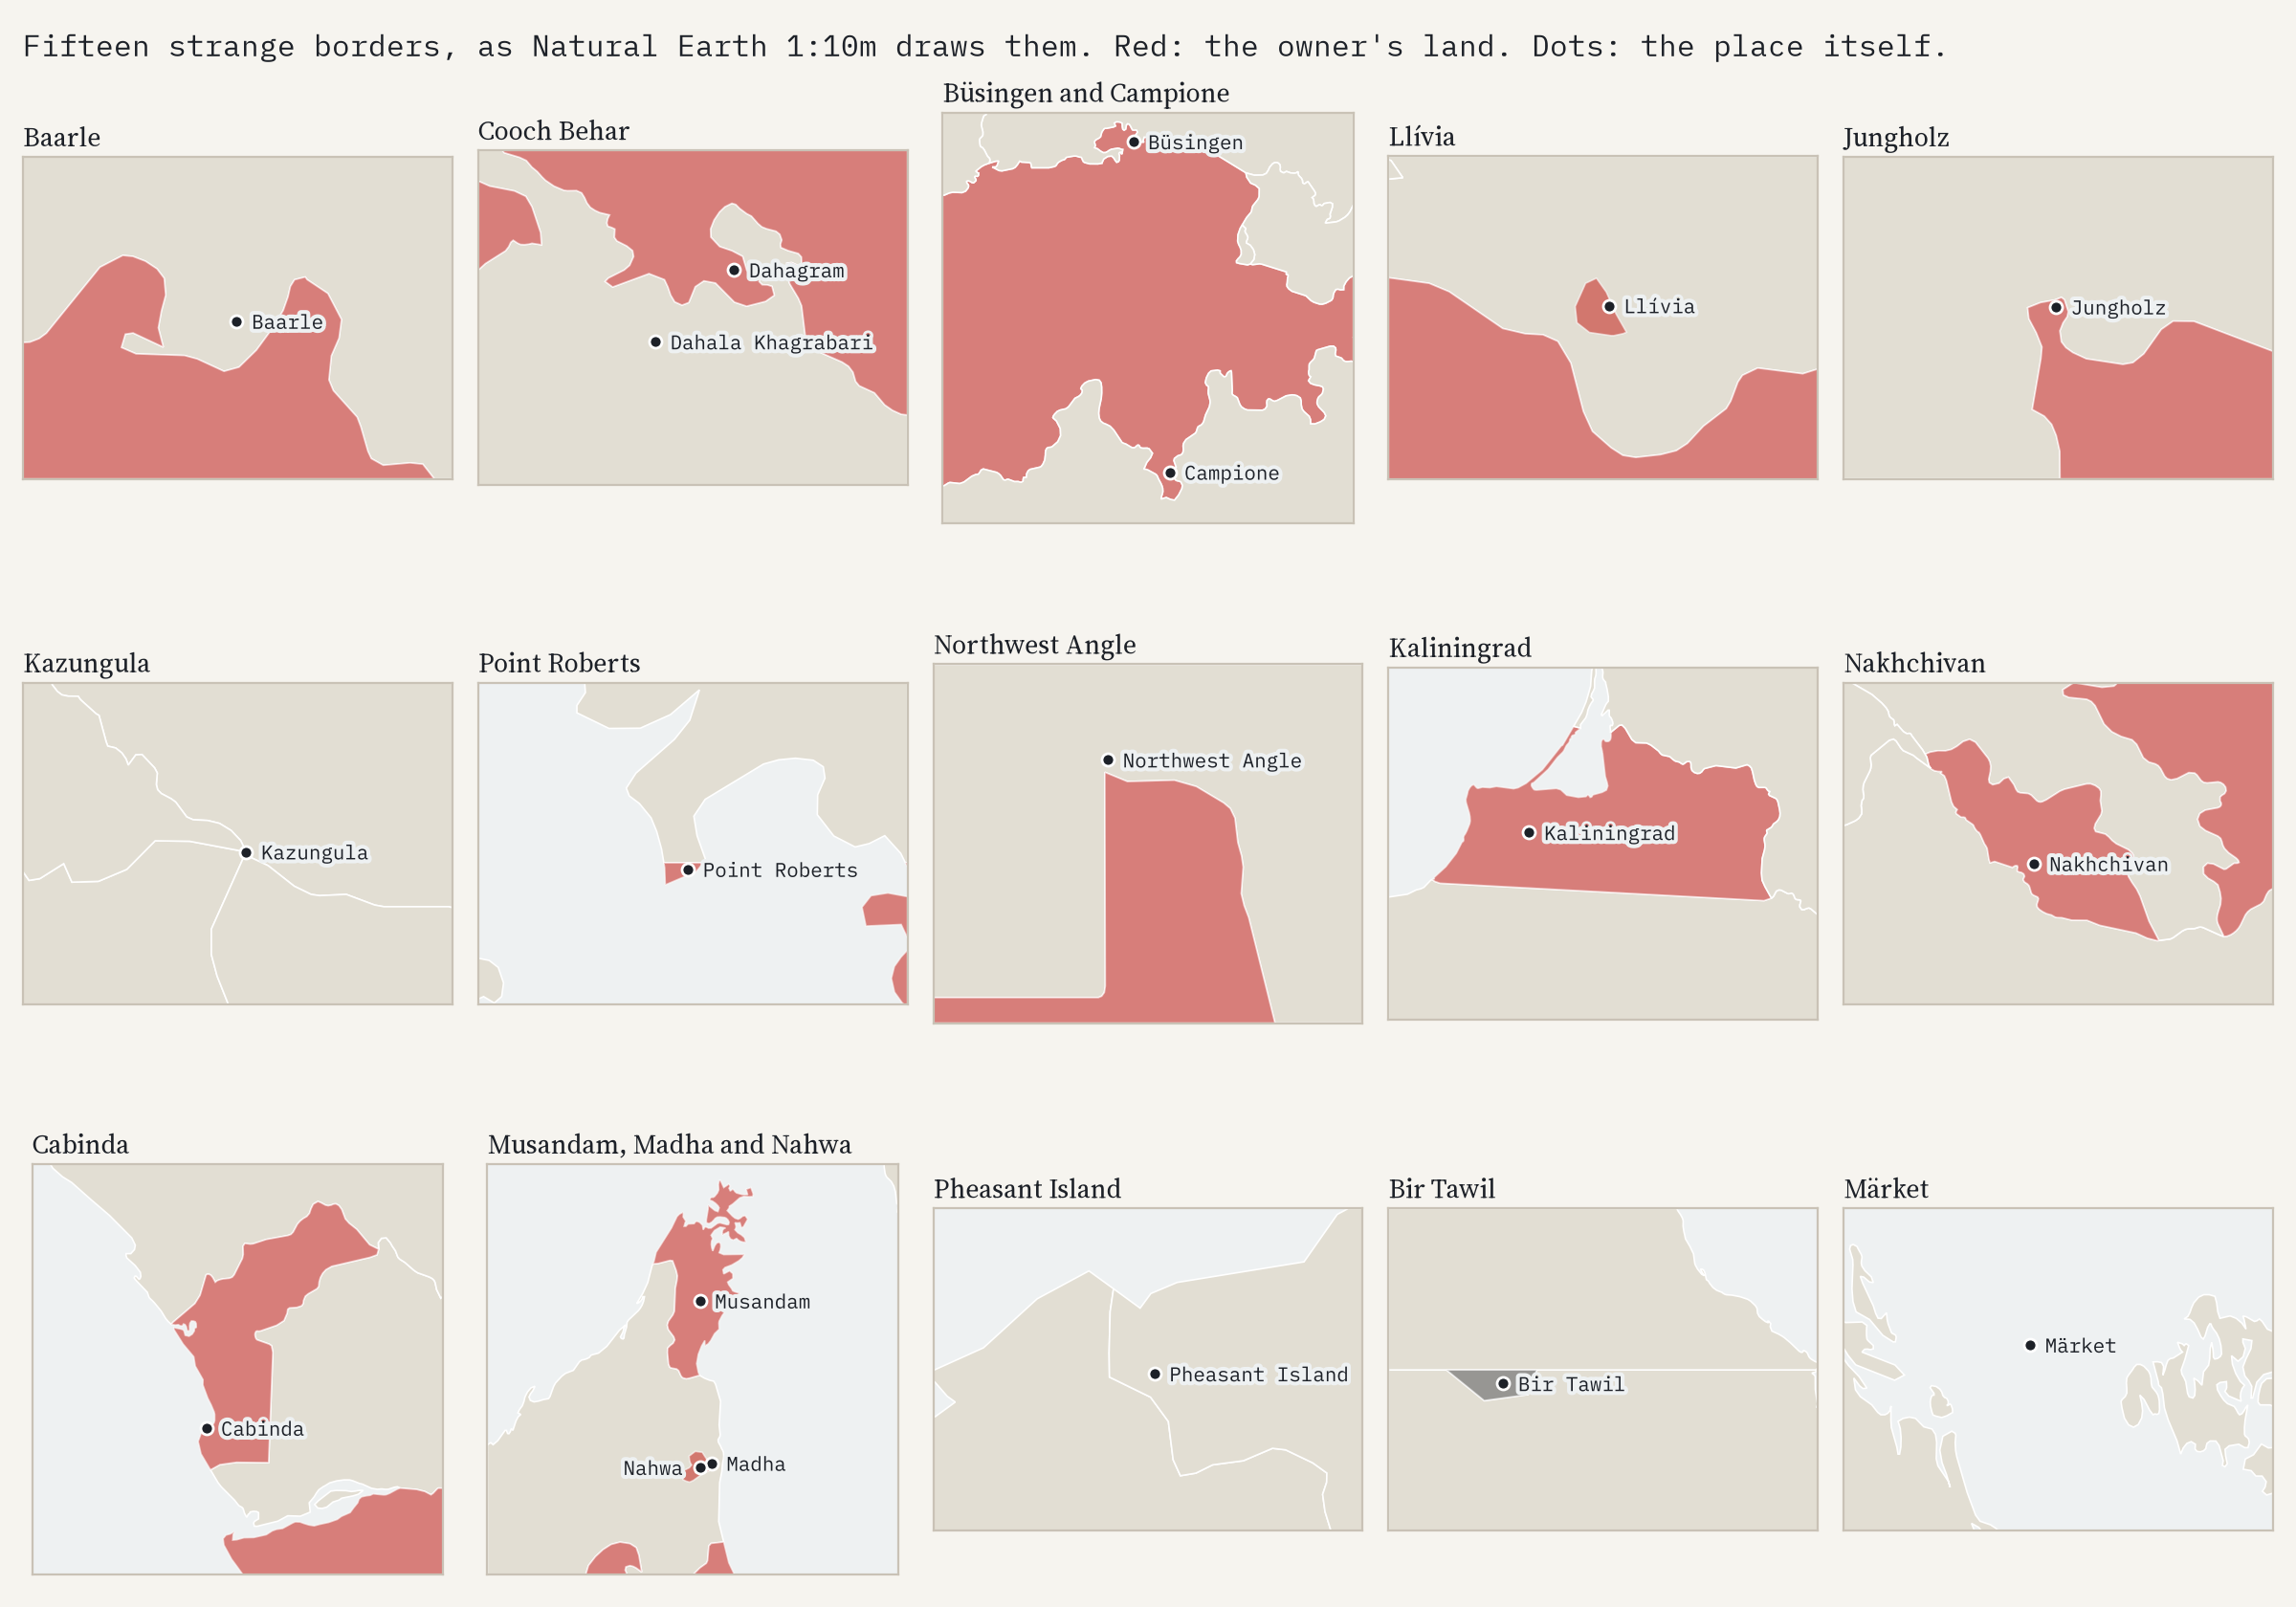
\includegraphics[width=\textwidth]{f_insets.png}
\caption{The 15 places on the tour, drawn from Natural Earth 1:10m. Shaded: the owner's land.}\label{fig:insets}\end{figure}

\subsection{Shared and unclaimed land}
Wikipedia's table lists 15 current condominiums \citep{wcondo}. The smallest and oldest is Pheasant Island (6,820 m²), shared by France and Spain since the Treaty of the Pyrenees of 1659 and administered by each in turn for six months \citep{wpheasant}. Bir Tawil (2,060 km²) is claimed by neither Egypt nor Sudan, because each claims the boundary that gives it the larger Halaib Triangle \citep{wbir}; on the Danube, four pockets including Gornja Siga are claimed by neither Croatia nor Serbia \citep{wnullius}. Märket, a 3.3 ha skerry, has been divided between Sweden and Finland since 1809, and its border was redrawn in 1985 to put its lighthouse in Finland with no net transfer of territory \citep{wmarket}.

\section{Limitations}
Wikipedia's list is a crowd-sourced catalogue; its categories overlap, some entries are disputed, occupied or de facto, and its areas are often rounded. I follow its wording and categories and do not adjudicate. Bulleted items vary in scope (one item can describe several places), so their counts are counts of list items. Natural Earth is generalised: a millimetre at 1:10m is 10 km on the ground, so small enclaves and short borders are lost, areas and lengths differ from official figures, and its lines are de facto. Detached pieces depend on how rivers and estuaries are drawn. The choice of each country's main piece is a rule, not a fact. Neither the sources nor this paper endorse any territorial claim.

\section{Conclusion}
A machine reading of the world map recovers the large and famous oddities, Kaliningrad, Nakhchivan, Cabinda, Musandam and Madha, the tripoints and the countries with the most neighbours, and it agrees with Wikipedia's counts of neighbours for nearly every country. But most true enclaves are too small for it, and where it disagrees with the written record the disagreement is usually an oddity in itself: a 150 m border, an island split in 2022, or a quadripoint that is really two tripoints. The strangest borders are best found by reading as well as by measuring.

\section*{Data and code availability}
The interactive map is at \url{https://maps.tristanhotham.com/border-oddities/}. Data and code are at \url{https://github.com/Tristan-Hotham/border-oddities} and archived with this paper at https://doi.org/10.5281/zenodo.23873011. Text, figures and derived data are released under CC BY 4.0, tables derived from Wikipedia under CC BY-SA 4.0, and code under the MIT licence. Natural Earth is public domain; Wikidata is CC0.

\section*{AI statement}
I wrote the text, with drafting and editing assistance from Claude (Anthropic), which also helped prepare the analysis code. I reviewed and checked all text and results.

\begin{thebibliography}{30}
\bibitem[Natural Earth(2026)]{naturalearth} Natural Earth (2026) Admin 0 countries (1:10m, 1:50m) and populated places (1:10m). Public domain. \url{https://www.naturalearthdata.com/}
\bibitem[Wikipedia(2026a)]{wlist} Wikipedia contributors (2026) List of enclaves and exclaves (revision 1378450919). CC BY-SA 4.0. \url{https://en.wikipedia.org/wiki/List_of_enclaves_and_exclaves}
\bibitem[Wikipedia(2026b)]{wenclave} Wikipedia contributors (2026) Enclave and exclave (revision 1379038567). CC BY-SA 4.0. \url{https://en.wikipedia.org/wiki/Enclave_and_exclave}
\bibitem[Wikipedia(2026c)]{wbh} Wikipedia contributors (2026) Baarle-Hertog (revision 1375646116). CC BY-SA 4.0. \url{https://en.wikipedia.org/wiki/Baarle-Hertog}
\bibitem[Wikipedia(2026d)]{wbn} Wikipedia contributors (2026) Baarle-Nassau (revision 1374958061). CC BY-SA 4.0. \url{https://en.wikipedia.org/wiki/Baarle-Nassau}
\bibitem[Wikipedia(2026e)]{wib} Wikipedia contributors (2026) Bangladesh-India enclaves (revision 1376307970). CC BY-SA 4.0. \url{https://en.wikipedia.org/wiki/Bangladesh-India_enclaves}
\bibitem[Wikipedia(2026f)]{wdahagram} Wikipedia contributors (2026) Dahagram-Angarpota (revision 1375726745). CC BY-SA 4.0. \url{https://en.wikipedia.org/wiki/Dahagram-Angarpota}
\bibitem[Wikipedia(2026g)]{wtri} Wikipedia contributors (2026) Tripoint (revision 1379426480). CC BY-SA 4.0. \url{https://en.wikipedia.org/wiki/Tripoint}
\bibitem[Wikipedia(2026h)]{wtrilist} Wikipedia contributors (2026) List of tripoints (revision 1367080204). CC BY-SA 4.0. \url{https://en.wikipedia.org/wiki/List_of_tripoints}
\bibitem[Wikipedia(2026i)]{wquad} Wikipedia contributors (2026) Quadripoint (revision 1381298137). CC BY-SA 4.0. \url{https://en.wikipedia.org/wiki/Quadripoint}
\bibitem[Wikipedia(2026j)]{wcondo} Wikipedia contributors (2026) Condominium (international law) (revision 1379384271). CC BY-SA 4.0. \url{https://en.wikipedia.org/wiki/Condominium_(international_law)}
\bibitem[Wikipedia(2026k)]{wnullius} Wikipedia contributors (2026) Terra nullius (revision 1380971148). CC BY-SA 4.0. \url{https://en.wikipedia.org/wiki/Terra_nullius}
\bibitem[Wikipedia(2026l)]{wlandlocked} Wikipedia contributors (2026) Landlocked country (revision 1377715267). CC BY-SA 4.0. \url{https://en.wikipedia.org/wiki/Landlocked_country}
\bibitem[Wikipedia(2026m)]{wland} Wikipedia contributors (2026) List of countries and territories by number of land borders (revision 1382121948). CC BY-SA 4.0. \url{https://en.wikipedia.org/wiki/List_of_countries_and_territories_by_number_of_land_borders}
\bibitem[Wikipedia(2026n)]{wone} Wikipedia contributors (2026) List of countries that border only one other country (revision 1379580410). CC BY-SA 4.0. \url{https://en.wikipedia.org/wiki/List_of_countries_that_border_only_one_other_country}
\bibitem[Wikipedia(2026o)]{wpheasant} Wikipedia contributors (2026) Pheasant Island (revision 1381049972). CC BY-SA 4.0. \url{https://en.wikipedia.org/wiki/Pheasant_Island}
\bibitem[Wikipedia(2026p)]{wbir} Wikipedia contributors (2026) Bir Tawil (revision 1377306827). CC BY-SA 4.0. \url{https://en.wikipedia.org/wiki/Bir_Tawil}
\bibitem[Wikipedia(2026q)]{wmarket} Wikipedia contributors (2026) Märket (revision 1383238902). CC BY-SA 4.0. \url{https://en.wikipedia.org/wiki/Märket}
\bibitem[Wikipedia(2026r)]{whans} Wikipedia contributors (2026) Hans Island (revision 1375816329). CC BY-SA 4.0. \url{https://en.wikipedia.org/wiki/Hans_Island}
\bibitem[Wikipedia(2026s)]{wmadha} Wikipedia contributors (2026) Madha (revision 1377951852). CC BY-SA 4.0. \url{https://en.wikipedia.org/wiki/Madha}
\bibitem[Wikipedia(2026t)]{wnahwa} Wikipedia contributors (2026) Nahwa (revision 1382973846). CC BY-SA 4.0. \url{https://en.wikipedia.org/wiki/Nahwa}
\bibitem[Wikipedia(2026u)]{wvenn} Wikipedia contributors (2026) Vennbahn (revision 1359463274). CC BY-SA 4.0. \url{https://en.wikipedia.org/wiki/Vennbahn}
\bibitem[Wikipedia(2026v)]{wother} Wikipedia contributors (2026) Articles used for the tour: Büsingen am Hochrhein (revision 1381375892); Cabinda Province (revision 1379291246); Campione d'Italia (revision 1380840280); Ceuta (revision 1381896212); Jungholz (revision 1376263980); Kaliningrad Oblast (revision 1382459682); Kleinwalsertal (revision 1380258009); Llívia (revision 1374532206); Melilla (revision 1381744763); Musandam Governorate (revision 1379359280); Nakhchivan Autonomous Republic (revision 1380806142); Northwest Angle (revision 1377833798); Point Roberts, Washington (revision 1382317302); Sankovo-Medvezhye (revision 1352277197). CC BY-SA 4.0.
\bibitem[Wikidata(2026)]{wikidata} Wikidata (2026) Items that are instances of enclave and related types. CC0. \url{https://www.wikidata.org/}
\end{thebibliography}
\end{document}
